\documentclass[border=0pt]{standalone}
\usepackage{fontspec}
\setmainfont{Carlito}
\usepackage{unicode-math}
\setmathfont{Latin Modern Math}
\usepackage{xcolor}
\usepackage{booktabs}
\usepackage{tikz}
\usepackage{graphicx}

\definecolor{canvabg}{RGB}{246,244,241}
\definecolor{textDark}{RGB}{40,40,40}
\definecolor{textMute}{RGB}{125,120,113}
\definecolor{accent}{RGB}{18,125,108}
\definecolor{trough}{RGB}{160,55,50}
\definecolor{bridge}{RGB}{30,90,140}

\pagecolor{canvabg}

\providecommand{\Cref}[1]{}
\providecommand{\cref}[1]{}
\providecommand{\ab}[1]{#1}

\begin{document}
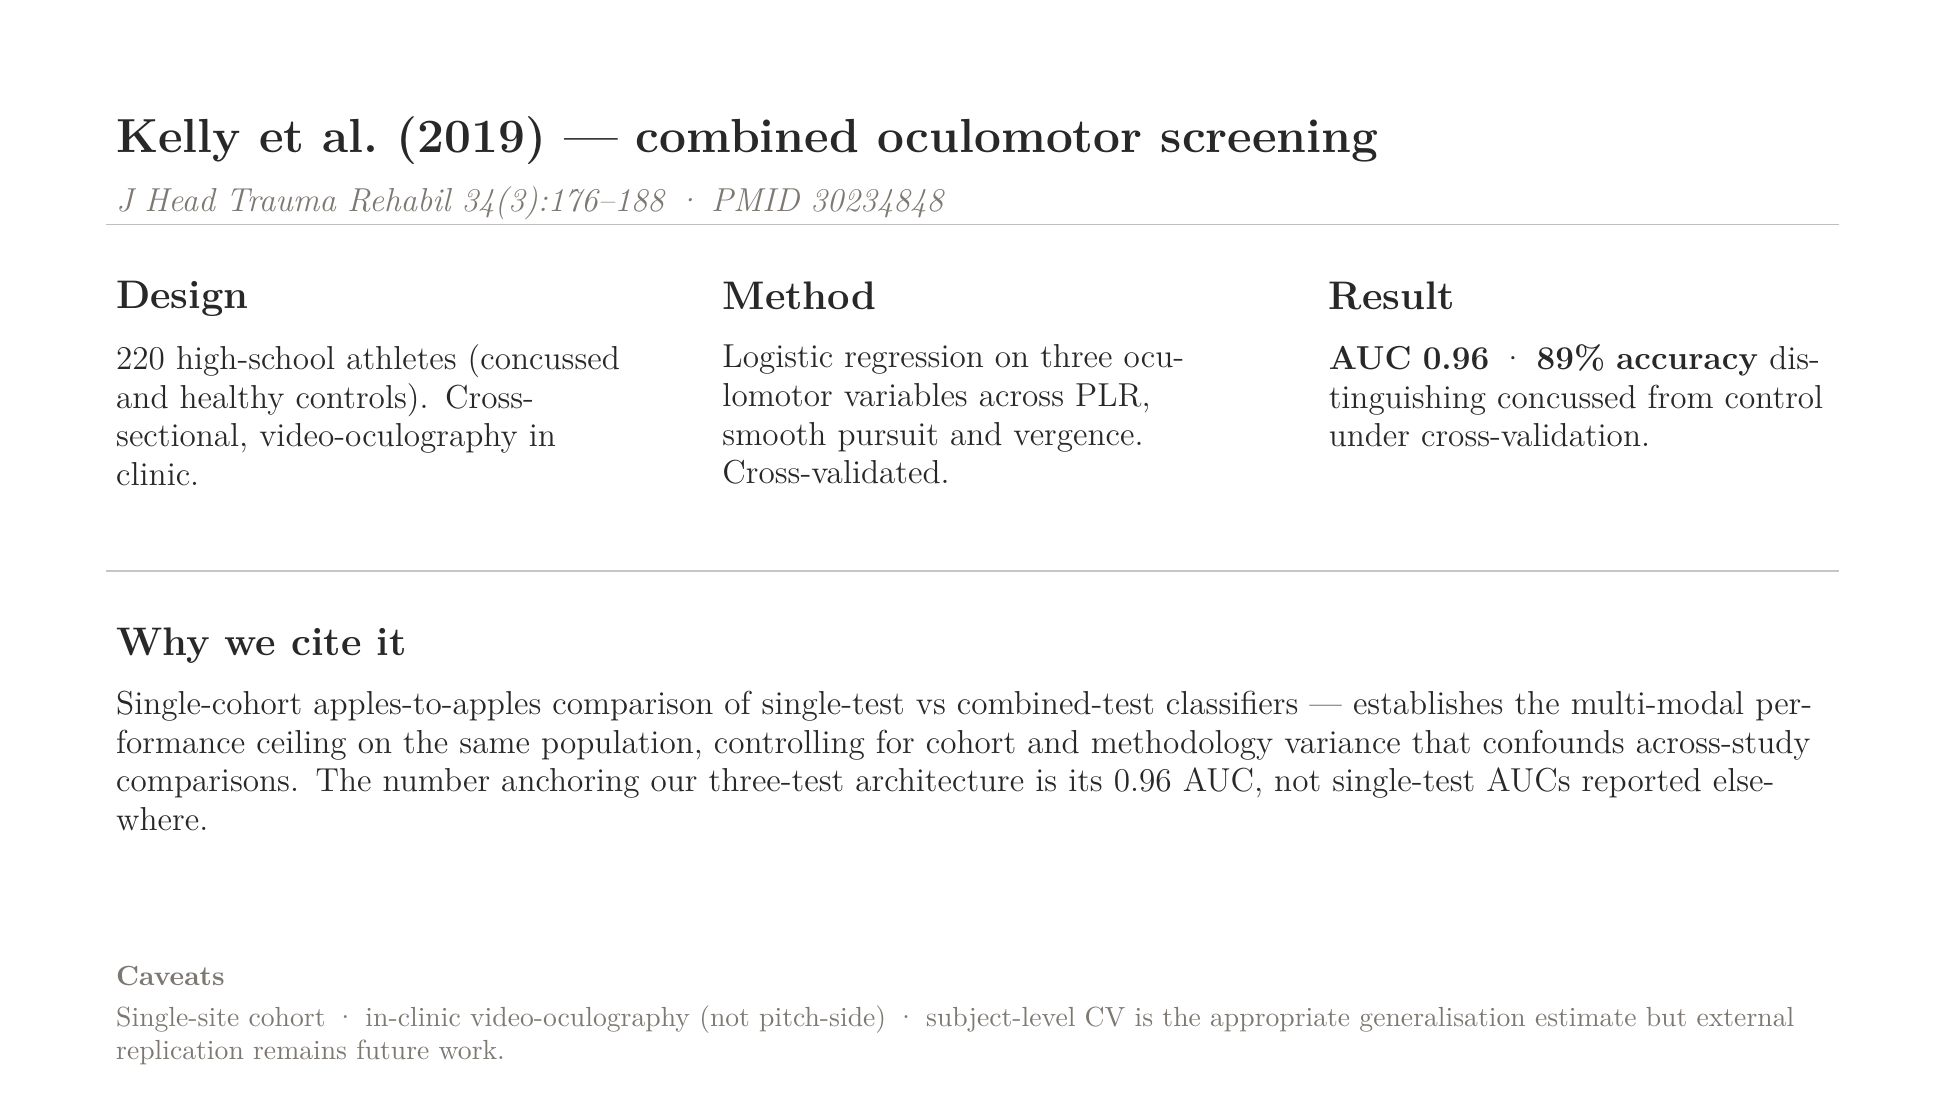
\begin{tikzpicture}[every node/.style={text=textDark}]
\useasboundingbox (0,0) rectangle (24, 13.5);

% Header
\node[anchor=north west, font=\bfseries\LARGE] at (1.0, 12.5)
    {Kelly et al.\ (2019) — combined oculomotor screening};
\node[anchor=north west, font=\itshape\large, text=textMute, text width=22cm]
    at (1.0, 11.6)
    {\textit{J Head Trauma Rehabil} 34(3):176--188 \textperiodcentered{} PMID 30234848};

\draw[gray!50, line width=0.5pt] (1.0, 11.0) -- (23.0, 11.0);

% Three-column body
\node[anchor=north west, font=\bfseries\Large] at (1.0, 10.4) {Design};
\node[anchor=north west, text width=6.5cm, font=\large] at (1.0, 9.6)
    {220 high-school athletes (concussed and healthy controls).
     Cross-sectional, video-oculography in clinic.};

\node[anchor=north west, font=\bfseries\Large] at (8.7, 10.4) {Method};
\node[anchor=north west, text width=6.5cm, font=\large] at (8.7, 9.6)
    {Logistic regression on three oculomotor variables across PLR,
     smooth pursuit and vergence. Cross-validated.};

\node[anchor=north west, font=\bfseries\Large] at (16.4, 10.4) {Result};
\node[anchor=north west, text width=6.5cm, font=\large] at (16.4, 9.6)
    {\textbf{AUC 0.96} \textperiodcentered{} \textbf{89\% accuracy}
     distinguishing concussed from control under cross-validation.};

% Why we cite
\draw[gray!45, line width=0.5pt] (1.0, 6.6) -- (23.0, 6.6);
\node[anchor=north west, font=\bfseries\Large] at (1.0, 6.0) {Why we cite it};
\node[anchor=north west, text width=22cm, font=\large] at (1.0, 5.2)
    {Single-cohort apples-to-apples comparison of single-test vs combined-test
     classifiers — establishes the multi-modal performance ceiling on the
     same population, controlling for cohort and methodology variance that
     confounds across-study comparisons. The number anchoring our
     three-test architecture is its 0.96 AUC, not single-test AUCs reported
     elsewhere.};

% Caveats
\node[anchor=north west, font=\bfseries, text=textMute] at (1.0, 1.7) {Caveats};
\node[anchor=north west, text width=22cm, font=\normalsize, text=textMute]
    at (1.0, 1.2)
    {Single-site cohort \textperiodcentered{} in-clinic video-oculography (not
     pitch-side) \textperiodcentered{} subject-level CV is the appropriate
     generalisation estimate but external replication remains future work.};

\end{tikzpicture}
\end{document}
